\chapter{Phénomène de localisation d'Anderson} %% Titre ?
%\begin{tikzpicture}[remember picture, overlay]
%\node[anchor=north east,inner sep=0pt] at (current page.north east) {
\includegraphics[scale=1]{Fig/Localisation/g825.png}};
%\end{tikzpicture}

présentation des effets d'interférences dans le désordre. scaling theory à la delande uniquement sur la conductance pour présenter la localisation 1D et 2D puis la 3D avec la transition. Terminer sur la quête du régime critique avec le graphe de delande2017, et introduction aux manips récentes et futures.


Paragraphe d'introduction? 

Dans ce chapitre, nous commencerons par décrire comment, lors de la propagation cohérente d'une onde dans un milieu désordonné, les interférences peuvent altérer la diffusion classique et engendrer le phénomène spectaculaire de \emph{Localisation d'Anderson} dont nous donnerons les principales propriétés. Dans un second temps, nous présenterons succinctement les principaux systèmes utilisés pour l'investigation de la localisation d'Anderson, pour s'attarder plus particulièrement sur les expériences d'atomes froids. Enfin, nous terminerons ce chapitre par une discussion de nos enjeux actuels, l'étude du régime critique de la transition d'Anderson, dont nous présenterons l'état de l'art.

\section{Diffusion et interférences}
\subsection{Phénomène de diffusion}
\label{sc:diffusion_classique}
Le phénomène de diffusion macroscopique est un phénomène de transport le plus connu de la physique classique. Celui-ci permet par exemple de décrire de manière simple la propagation de la chaleur dans un matériau homogène, l'homogénéisation de la concentration de particules dans un liquide ou encore le phénomène de résistance électrique dans un cadre unifié. 

En effet, le phénomène macroscopique de diffusion provient, de manière générale, d'une marche aléatoire des particules vectrices au sein de leur environnement. Drude a ainsi été le premier à calculer la résistivité électrique des matériaux en introduisant un temps de relaxation basé sur les collisions entre les électrons, vecteurs du courant électrique, et les impuretés du matériau dans lequel ceux-ci se déplacent \citep{ashcroft2010solid}. 

Il apparaît ainsi que certaines propriétés macroscopiques des matériaux sont reliées aux grandeurs caractéristiques de la marche aléatoire associée. Ces grandeurs sont des briques élémentaires de la propagation en milieu désordonné, telles que le temps de diffusion élastique, le temps de transport, ou encore le coefficient de diffusion, que nous présenterons dans la suite.

\paragraph*{Temps de diffusion élastique}
La quantité la plus naturelle permettant de caractériser de manière microscopique le phénomène de diffusion est le \emph{temps de diffusion élastique} $\taus$, qui correspond à la durée typique entre deux évènements successifs de \emph{collision élastique} avec les impuretés du milieu. Ce temps est l'équivalent temporel du \emph{libre parcours moyen}  $\ls$ correspondant à la distance moyenne entre deux évènements de diffusion microscopique successifs. Dans le cas d'une particule de masse $m$ se déplaçant à une vitesse $v_{\mathrm{i}}$, ces deux grandeurs sont reliées par
\begin{equation}
\taus=\frac{\ls}{v_{\mathrm{i}}}=\frac{m}{\hb} \frac{\ls}{k_{\mathrm{i}}} \text{ ,}
\end{equation}
où $k_{\mathrm{i}}$ est le nombre d'onde de l'onde quantique associée à la particule (celui-ci est inchangé après chaque évènement de collision en raison de leur caractère élastique). 

Comme nous le verrons plus en détails dans les chapitres \ref{ch:TauS_PRL} et \ref{ch:TauS_NJP}, le temps de diffusion élastique est une quantité qui dépend des détails microscopiques du système, établissant ainsi le lien entre processus microscopiques et phénomène macroscopique.


\paragraph*{Temps de transport}
Si la norme du vecteur vitesse (ou de manière équivalente du vecteur d'onde) reste inchangée au cours de la propagation, sa direction est modifiée à chaque évènement de collision élastique. Comme nous le verrons plus en détails dans le chapitre \ref{ch:TauS_PRL}, lors de la collision avec un diffuseur de taille caractéristique $\sigma$, l'onde peut être diffusée selon un angle $\left\langle\theta\right\rangle\sim 1/k_{\mathrm{i}} \sigma$. La diffusion peut donc être \emph{anisotrope}, analogie avec la diffraction en optique.

En considérant que la trajectoire d'une particule est composée de multiples collisions, il apparaît alors une seconde échelle de temps caractéristique, le \emph{temps de transport} ou temps de Boltzmann $\taub$, décrivant la durée nécessaire pour la particule perde l'information de la direction initiale de sa vitesse. 


On peut ainsi montrer que le temps de transport (et son analogue spatial, la \emph{longueur de transport}) s'expriment en fonction du temps de diffusion élastique \citep{akkermans2007mesoscopic}
\begin{equation}
\taub=\frac{\taus}{1-\left\langle\cos{\theta}\right\rangle} \quad \text{et} \quad \lb=\frac{\ls}{1-\left\langle\cos{\theta}\right\rangle} \text{ ,}
\end{equation}
où $\langle\dots\rangle$ représente la valeur moyenne sur les différents évènements de diffusion.


\begin{figure}
\centering

\caption{\textbf{Stuff.} Stuff.}
\label{fig:diffusion_classique}
\end{figure}

\paragraph*{Coefficient de diffusion}
coefficient de diffusion





\subsection{Localisation faible}
\label{sc:weak_localisation}
effets d'interférences qui résistent à la réalisation du désordre augmentent la probabilité de revenir à l'origine.
calcul sur les amplitudes de diffusion: CBS et localisation faible.
$D\rightarrow D-\delta D$
\begin{equation}
\delta D/ D_{\mathrm{B}} = \left\lbrace \begin{aligned}
& \mathcal{O}\left(L/l_{\mathrm{B}}\right)  \quad &&\text{en 1D}\\
& \mathcal{O}\left(\frac{1}{k l_{\mathrm{B}}} \ln{\frac{L}{l_{\mathrm{B}}}} \right) \quad &&\text{en 2D}\\
& \mathcal{O}\left(\frac{1}{(k l_{\mathrm{B}})^2}\right) \quad &&\text{en 3D}
\end{aligned}\right.
\end{equation}

\subsection{Suppression du transport: Localisation d'Anderson}
\label{sc:localisation_anderson}
suppression du transport $D=0$. profil exponentiel de la fonction d'onde. longueur de localisation.
1D et 2D toujours localisé sur différentes tailles. existence d'une transition de phase en 3D, régime critique.
%\subsection{Théorie d'échelle}

\section{Localisation des atomes froids}
\subsection{Etudes expérimentales de la localisation d'Anderson}
phénomène universel, commun à tous types d'ondes.
ultrasons, lumières dans des guides d'onde désordonnés, lumière dans la peinture blanche, ondes électroniques dans des matériaux dopés


\subsection{L'approche des atomes froids}
parler ondes de matières dans des potentiels lumineux. du coup on contrôle tout, même la dimensionalité. 
expérience de diffusion de à 2D (équipe de thomas), qui montre la décroissance du  pic central en 1/t ou 1/t2 suivant désordre ou non.

parler des manips 1D qui démontrent la localisation. Introduire $\sigma$ la taille des grains pour expliquer le effective mobility edge?

Parler des manips préliminaires à 3D. 

Introduire brièvement le many-body, kick-rotors?
expérience récente en 2D.

\section{Vers l'étude du régime critique}
\subsection{Etat de l'art de l'étude de la transition d'Anderson}
\lipsum[6]
\subsection{Nécessité d'une spectroscopie pour sonder le régime critique}
\lipsum[7]







\begin{comment}
%% TODO: finir introduction (lep lus importantp our bien savoir quoi écrire par la suite
%% TODO: vérifier que ce qui a déjà été écrit est cohérent avec le reste

%Chapter 1: Introduction - Etat de l'art
%-----------------------

%1.1: Prise de décision: pt de vue cognitif et neuroscience
%-
%-
%-

%1.2 : differents modèles de prise de décisions
%- SDT %% rapidement seulement
%- Seq. Analysis
%- Attractor models %% equation du modèle qu'on va utiliser


%1.3 : variété d'effets testés dans ce type de tache
%- Biais de répétitions
%- Fréquence des stimulis
%- Reinf learning

%% Intro générale ici
Decision-making is vital for human and animal behaviors. It involves choosing an action or an option among multiples alternatives using different information such as sensory inputs, past associations and future goals. Decision-making has been studied in various fields, such as psychology, statistics, economics, finance, political science, philosophy, ethics and jurisprudence. %% REFS TODO important
The last two decades have seen a  surge of interest in the neurobiological studies of decision-making thanks to animal behavioral physiology, human brain imaging and neural circuit modelling. In this chapter I will review the neuronal underpinning of decision-making and different models that have been proposed. %% est-ce que je fais raiment ça au final ? si je ne parle pas de toute la biblio
Finally, I will trouver la bonne formulation. %% TODO



%% Que faire des article Katz et al ? en conclusion ou bien en intro ?
%% Les descriptions sont-elles assez claires ? plus de descriptions ????
%% penser à l'article XJ sur la saccade


\section{Decision-making in cognitive science and neuroscience}
%% a faire après
%% trouver bonne review ou mail jérôme ?
%% ou inclure cog et neuro en même temps

A central idea to decision-making is time integration. The idea of temporal accumulation of evidence has a long history in cognitive psychology. Decision-maker typically take longer times to perform more difficult decisions~\citep{hick1952rate,vickers1970evidence}, and there is a tradeoff between speed and accuracy, i.e performances improve with slower response times~\citep{wickelgren1977speed}.
%% on parle des RTS ???
%% puis de la différence humain animaux
%% puis neuronal ??? faire attention au plan et citations
However, it is not obvious to determine the timescale on which this accumulation of evidence occurs~\citep{uchida2006seeing}.  

One of the most-studied perceptual decision task is the random dot motion task. Participants (humans or monkeys) look at a screen where some dots are moving randomly and the others coherently into one of the two possible directions. The participants must report the net direction of motion by making a saccade in this direction. %% à modifier ?
When the fraction of dots moving coherently is reduced, the decision becomes more difficult. In this task, when the difficulty is varied, reaction times can go from $300$~ms to the order of the second. %ù TODO REFS
The two-alternative-forced-choice (2AFC) task %% faut-il préciser ce que sait ou bien on comprend de précedemment ?
has been studied in rodents too, in the case of an olfactory discrimination. %% REFS
In such tasks, the rats needed to respond to the dominant component in binary odour mixtures. The first observation is that these decisions are fast, around $300$~ms. The performances varied from chance level to almost $100 \%$ correct with the stimulus difficulty. However, the difference in reaction times between the easiest and the hardest stimuli is smaller than for humans and monkeys, around $35$~ms in~\cite{uchida2003speed}  and $80$~ms in~\cite{abraham2004maintaining}. These different results highlight the diversity of time integration across tasks and species.

Electrophysiological studies in behaving monkeys have been performed in order to understand the neural mechanisms underlying perceptual decision-making. %% REFS et exemple figure tache
Research has focused on cortical neurons  that encode task-relevant sensory signals in different perceptual decision-making tasks, such as the random dot motion task or sensorimotor tasks (Figure~\ref{fig:RDM}.A). %% REFS et fig.

%%% mettre les performances ??? ceci peut être intéressant ? chercher données ? Freedman peut être ?
\begin{figure}[h!]
	\centering
	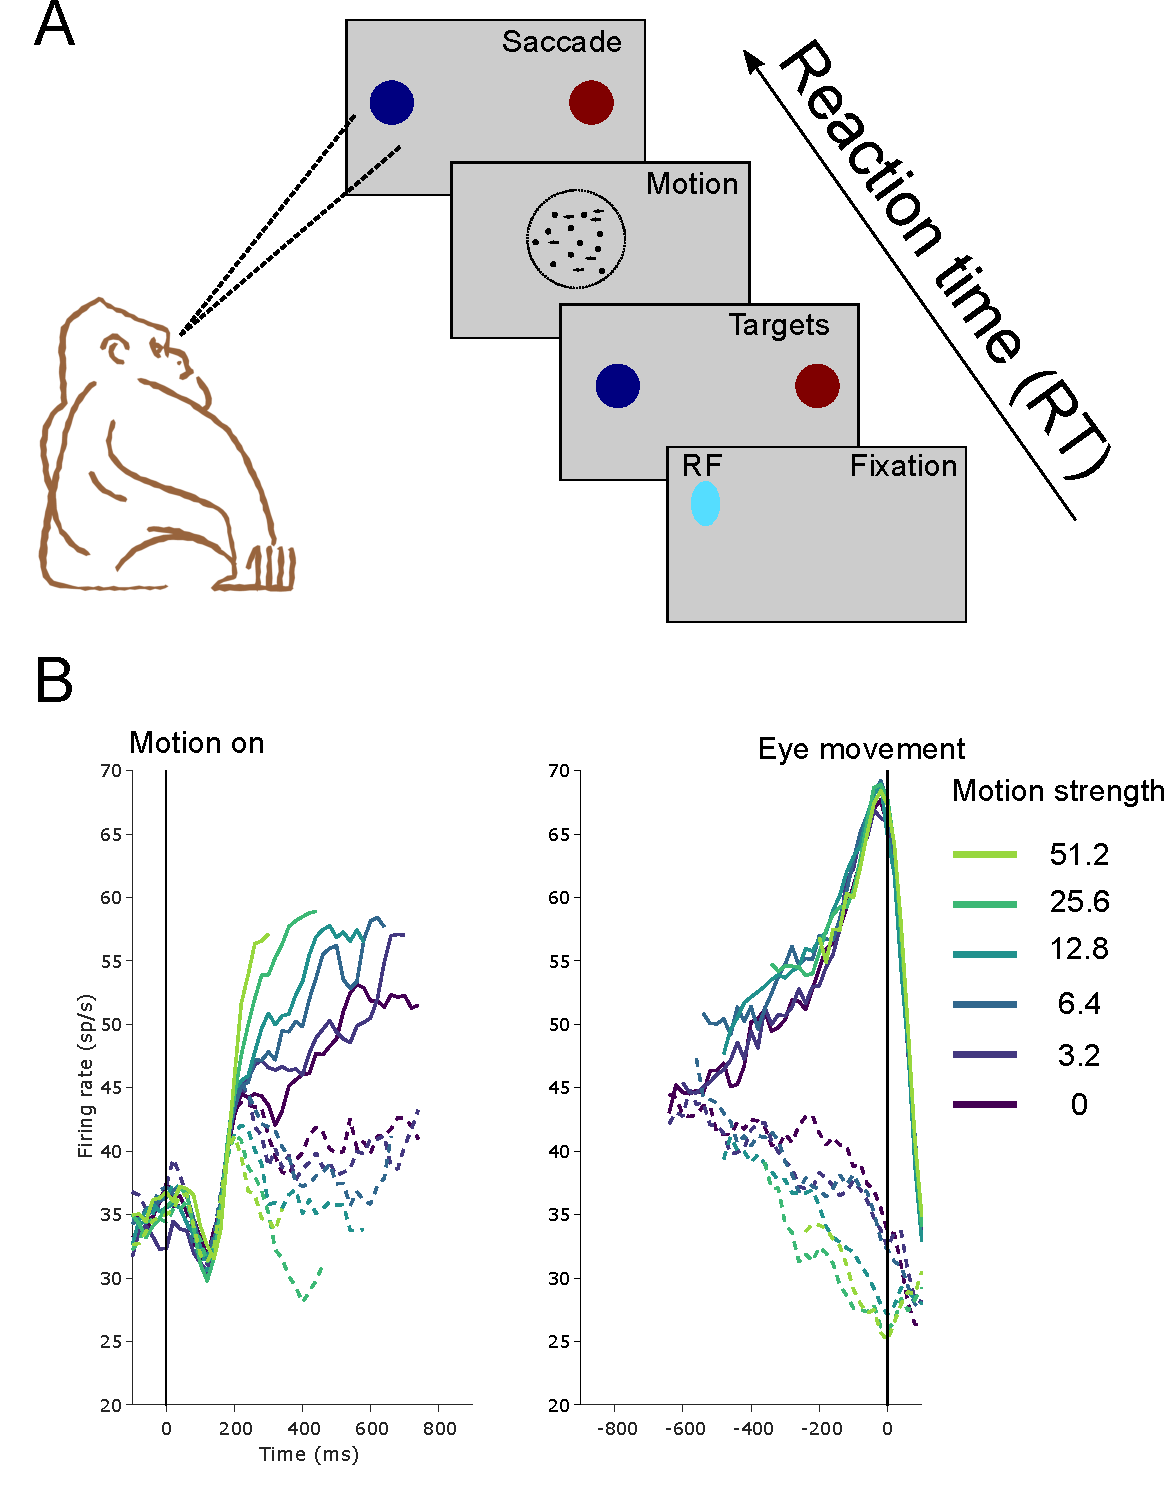
\includegraphics[width=0.8\linewidth]{Fig/Chapter1/RDM.pdf}
	\caption{{\bf Reaction time version of the random dot motion discrimination task.}   (A) The monkey views a set of dots moving across the screen and decides the net direction of movement. The decision is indicated by a saccadic eye movement to one the two peripheral target. The light blue field corresponds to the receptive field of one of the recorced LIP neurons. The monkey is the figure was obtained using the AutoDraw software. (B) Response of LIP neurons during decision. The data are from~\cite{roitman2002response} and are publicly available. The average firing rate of $54$ LIP neurons is shown for $6$ degrees of difficulty. The firing rate are grouped by motion difficulty and direction of choice (dashed line corresponding to choice out of the receptive field of the neuron). The left panel represents the average firing rate during decision formation starting from motion onset. The right panel shows the average firing rate centered at the time of the eye movement.
	}
	\label{fig:RDM}
\end{figure}
%% REF AutoDraw ??,



%In the following part I will focus on the random dot motion discrimination task. %% ou pas ? ce sera pas au final
%https://www.sciencedirect.com/science/article/pii/S0896627308008362#bib77
Sensory neurons in the visual area MT encode the motion direction of the stimulus~\citep{newsome1989neuronal,britten1992analysis,britten1993responses}, but the decision process does not occur in this area. %% exemple des perfomances des singes dans ces taches ?
\cite{shadlen1996motion} found that the activity of neurons in the lateral intraparietal cortex (LIP) %% check les différentes donénes en ligne
was correlated with the monkey's perceptual choice. Moreover, in reaction time version of the task (when response times are controlled by the monkeys), a number of findings suggest that LIP neurons mediate decisions between rival saccadic decisions~\citep{roitman2002response,huk2005neural,gold2007neural,huk2012neural}. The activity of the LIP neurons selective for the saccadic target increased from the stimulus onset until the saccadic eye movement (Figure~\ref{fig:RDM}.B). This buildup rate depends on the quality of the sensory of information, with stronger evidence associated to steeper slopes. Finally, %% effect of micro stim. https://hankslab.faculty.ucdavis.edu/wp-content/uploads/sites/305/2017/02/Hanks_Summerfield-Neuron2017.pdf
the decision choice is made when the firing rate of the LIP neurons (corresponding to this choice) reaches a threshold that is independent of the signal quality and of the response time.
In addition, microstimulations on MT and LIP neurons have an effect on accuracies and reaction times consistent with the idea that LIP neurons integrate sensory information~\citep{ditterich2003microstimulation,hanks2006microstimulation}. 
These different studies support the notion that LIP neurons act as a neuronal intergator by displaying stochastic ramping of activity. %ù ccl à revoir ?

%e RDM task
%showed that microstimulation of directionselective MT neurons causes monkeys to bias
%their decisions in favor of the preferred direction of the stimulated neurons (Salzman et al.


%% conclusion sur LIp neurons etc comme intergateurs.
%%% surement trouver d'autres choses à dire
%% peut être les arguments contre ?
%% sensorimotor tasks
%% recent experiments

%There is debate about where exactly the accumulation takes place, but it is clear that (at least) LIP, FEF, and SC form part of a circuit that is involved in implementing oculomotor decisions in monkeys performing simple decision-making tasks. The above studies generally support the notion that decision-related information flows from LIP to FEF and then to SC just prior to a decision.



\section{How can decision-making be modelled ?} %titre

Many models have been proposed to explain decision-making in humans and animals. There are two categories of models: dynamical models and non-dynamical models. Here, I will focus on dynamical models as they are more adequate to model the neuronal dynamics during decision-making.


\subsection{Drif-diffusion model}
Abstract mathematical tests have been developped to decide between two hypotheses, such as the sequential probability test. %% REFS
This test is optimal in the sense that it achieves a desired error rate with the minimum mean decision time. According to this test, decisions are initiated when cumulative estimates of noisy evidence variables reache a specific threshold. %ù REFS  race etc
The most-used model within the race framework is the drift-diffusion model (DDM). It consists in an unique integrator that accumulates the difference between the evidences for the two alternatives. The choice is made when the level of activity of the integrator exceed a specific threshold, positive or negative depending on the alternative (Figure~\ref{fig:DDM}). %ù figure

\begin{figure}[h!]
	\centering
	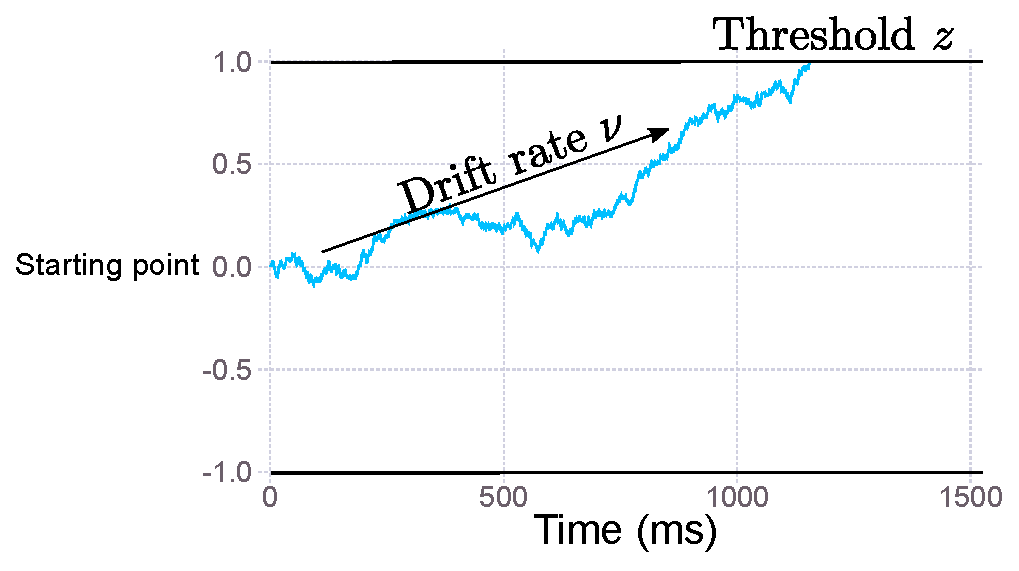
\includegraphics[width=0.8\linewidth]{Fig/Chapter1/Example-DDM.eps}
	\caption{{\bf Drift diffusion model.} Example of the dynamics of the diffusion model. The two black lines denote the threshold $z$ and $-z$ corresponding to the two alternatives. The race is ended when it reaches one of the two boundaries. In this example, the decision made correspond to a correct trials as the drift rate $\nu$ was chosen positiv.   
	}
	\label{fig:DDM}
\end{figure}


The success of the DDM framework is that it can decompose observed choice behavior into a cognitive process. As a dynamical model, it takes into account decision accuracies and response times and can address the speed-accuracy tradeoff. DDM will integrate for a shorter time if the evidence for the winning alternative is strong with respect to the losing alternative. Respectively, it will take longer time to reach a decision if the difference of evidence is small. The model is based on the following parameters. The starting point $a$ of the evidence accumulation represents a possible bias for one of the two alternative. This accumulation is performed at a certain drift rate $\nu$ and is related to the quality of information present within the stimulus. Typically, in the RDM experiment, this parameter would differ depending on the strength of the dots motion. The boundary represents the level of caution, the more this parameter is high, the less the model is making the wrong choice. Finally, the last parameter consist in the non-decision times that are an additive lag representing the motor lag of the participants for example. %% REFS

DDM have been succesfully used to account for behavioral data in a wide-range of decision-making paradigms. %% REFS
One should note that DDM does not only reproduce the error rates and response times, but the shape of the response times (RTs) too. %ù REFS
However, it is necessary to add across-trial variability for the different parameters in order to correctly model the RTs distributions of correct and error trials. Otherwise, due to the linearity of the model, the shapes of these distributions are strictly identical which is not what experimental studies have found. % REFS



\subsection{Recurrent cortical circuit}
There are two major critics that can be made about the DDM framework, when the goal is to model neural activity during decision-making. First, neural activity is non-linear (Figure~\ref{fig:RDM}.B) but the DDM is strictly linear. Secondly, DDM have no biophysical foundations and do not explain how this integration mechanism is implemented in the brain. Different models have been proposed to account for the cortical processes of decision-making: \cite{shadlen2001neural,usher2001time,wang2002probabilistic}.
I will focus on the approach of \cite{wang2002probabilistic}, as the two other models consist more in extension of the DDM framework.

\paragraph*{Attractor network}
Neurons in LIP and prefrontal cortex have shown to display directionally tuned activity~\citep{gnadt1988memory,funahashi1989mnemonic}. This suggests that a commun mechanism could underlie working memory and decision-making. One mechanism to generate persistent activity similar to working memory is the one of strong recurrent excitation in a local cortical circuit that will give rise to stimulus-selective attractor states~\citep{freeman1995hebbian,goldman1995cellular,brunel2001effects}. \cite{wang2002probabilistic} applied a biophysically based model to simulate the random dot motion discrimination task. In this model, the intergration is achieved through a mix between feedback excitation (N-methyl-D-aspartate (NMDA) channels with relatively long time constants) and inhibitory mechanism. Later, this model has been reduced to a mean-field version that is much faster to simulate~\citep{wong2006recurrent}. The model consists of two neuronal pools with subpopulations of spiking neurons selective for the two choices, denoted by $C_1$ and $C_2$ (Figure~\ref{fig:att-net}.A). The two neural populations compete with each other through feedback inhibition from interneurons. Both selective neural populations receive conflicting sensory inputs, with the motion strength characterized by the quantity $c$ (called coherence level).
%% fig à  insérer doit-elle celle du modèle original de Wang 2002 ?
%% plus de détails sur les courants et sur la description ???

\begin{figure}[h!]
	\centering
	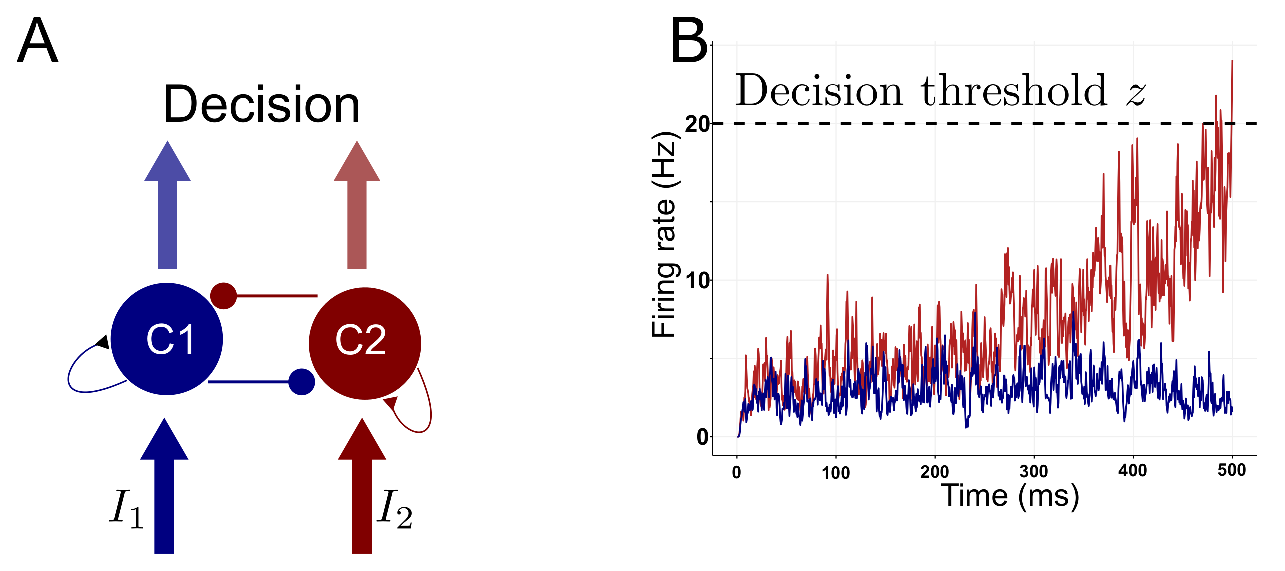
\includegraphics[width=0.8\linewidth]{Fig/Chapter1/attractor-network.eps}
	\caption{{\bf Attractor neural network of~\cite{wong2006recurrent}.} (A)  Schematic version of the local circuit of decision-making. Two neural pools ($C_1$ and $C_2$) compete with each other through lateral inhbition and are subject to recurrent excitation. This model corresponds to the mean-field version of~\cite{wang2002probabilistic}. (B) Dynamics of the network during decision-making process. Each neural population shows a ramping up of activity until one of the two wins the competition and reaches the decision threshold. In this case, the winnning population is $C_2$ and corresponds to the choice made by the network.
	}
	\label{fig:att-net}
\end{figure}

Figure~\ref{fig:att-net}.B represents an example of the dynamics of this model. At the stimulus onset, the firing rates of the two populations lie together and ramp up until they diverge from each other. The divergence is due to the winner-take-all dynamics that occurs in this network through recurrent excitation and feedback inhibition. The choice is based on which population wins the competition. In the reaction time version of the task, this is indicated by the fact that one of the two populations crosses a fixed threhsold (Figure~\ref{fig:att-net}.B).

%% un mot sur diagramme de bifurcation et pourquoi ceci donne WM et autre.



\paragraph*{Modelling behavioral data}
Attractor neural networks have been shown to account for many of the behavioral results. Figure~\ref{fig:rt-perf} shows the variation of accuracies and reaction times with respect to motion strength. As expected, the strongest is the stimulus, the slower is the decision time of the model. This is due to the fact that stronger stimuli lead to a stronger ramp up of activity. As mentionned previously, to obtain the different shapes of RTs distributions for correct and error trials within the DDM framework, one needs to implement a variabality of the parameters across trials. One key feature of attractor network is that this difference in distribution is naturally present. Figure ??? represents the decision process in the phase-plane space (firing rates of population $A$ against population $B$). When the decision is in favor of $A$, the basin of attraction corresponding to this attractor is larger, denoted by the ? line. The system starts naturally in the basin of attraction of $A$. To make the wrong decision, it would need to cross the boundary between the basins. Crossing a boundary between basins of attraction is a slow processus, and that explains why the reaction times are slower in error trials than for correct trials. % REFS
In contrast, a neural implementation of the diffusion model would yield the opposite effect~\citep{mazurek2003role}. %% ccl à changer ?
Another major difference between diffusion model and attractor neural network consists in the behavior at long duration of stimulus. \cite{kiani2008bounded} performed a motion discrimination task in monkeys but with variable stimulus duration. They found that performances reach a plateau when duration of stimulus increase. This phaenomen is not consistent with the DDM framework as performance can improve indefinitevely with stimulus time. In contrast, performances are bounded for long stimulus durations in the atrtactor neural network~\citep{wang2002probabilistic} as the ramping activity finally reach an attractor state.

\begin{figure}[h!]
	\centering
	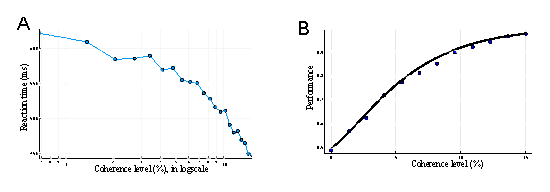
\includegraphics[width=0.8\linewidth]{Fig/Chapter1/perf-acc.eps}
	\caption{{\bf Behavioral performances of the attractor neural network.} (A) Reaction times of the circuit with respect to coherence levels. The coherence level is the variable $c$ and represent the difference in motion strength that arrives at both units.   (B) Performance of the model with respect to the coherence level.
	}
	\label{fig:rt-perf}
\end{figure}


%% ccl ????


\paragraph*{Successes of cortical circuits models}

%% voir article Wang

%% intro de la phrase à revoir
%% igure wong 2007 à refaire ????
One advantage of using attractor neural network to model decision-making is that it can be used to look more closely at the neuronal process of decision-making.  First, in Figure~\ref{fig:RDM}.B one can observe a drop in the firing rate of the LIP neurons before the ramping up of activity. The same behavior can be observed in attractor networks~\citep{wong2007neural}. In this study, the authors studied the influence of new arriving evidence during a decision process. They found that the influence diminishes over time, an effect that has been observed in monkeys experiment too~\citep{huk2005neural,wong2007neural}. This time-shift invariance can not be accounted for by diffusion models, as such models predict in fact the opposite effect~\citep{wong2007neural}.


In the attractor neural network, recurrent excitation must be balanced by feedback inhibition. This is mediated by lateral synaptic inhibition between the neural pools. In a monkey experiment, \cite{hanks2006microstimulation} performed microstimulation of LIP neurons selective to direction. They found that not only the decision towards the preferred direction was faster, but it slowed down the decision in the opposite direction too. This observation is consistant with a recurrent neural network with feedback inhibition. Attractor neural networks have not just been developped for the random dot motion discrimination task but for the somatosensory discrimination too. %ù REFs
It has been shown that reciprocal inhibition between two neural pools could exhibit persistent activity as observed in prefrontal neurons. %% REFS
Moreover, this circuit can perform the discrimination computation, e.g $f_1 > f_2$, during the comparison period. %% REFS

One limit to both diffusion models and the attractor neural network I presented is the biological substrate of decision threshold. Before a saccade is made (in the case of an occolumotor task), neurons in the frontal eye field (FEF) and superior colliculus (SC) fire a burst of spikes~\citep{hanes1996neural,munoz2002vying}.
These neurons are selective of saccade amplitude and direction. Using the initial framework of the attractor neural network, \cite{lo2006cortico} have studied an extended version of this circuit that involves the termination of the decision process. %% FIG ???

%% TODO: simulation du réseau Lo Wang saccade
\begin{figure}[h!]
	\centering
	% formu à changer
	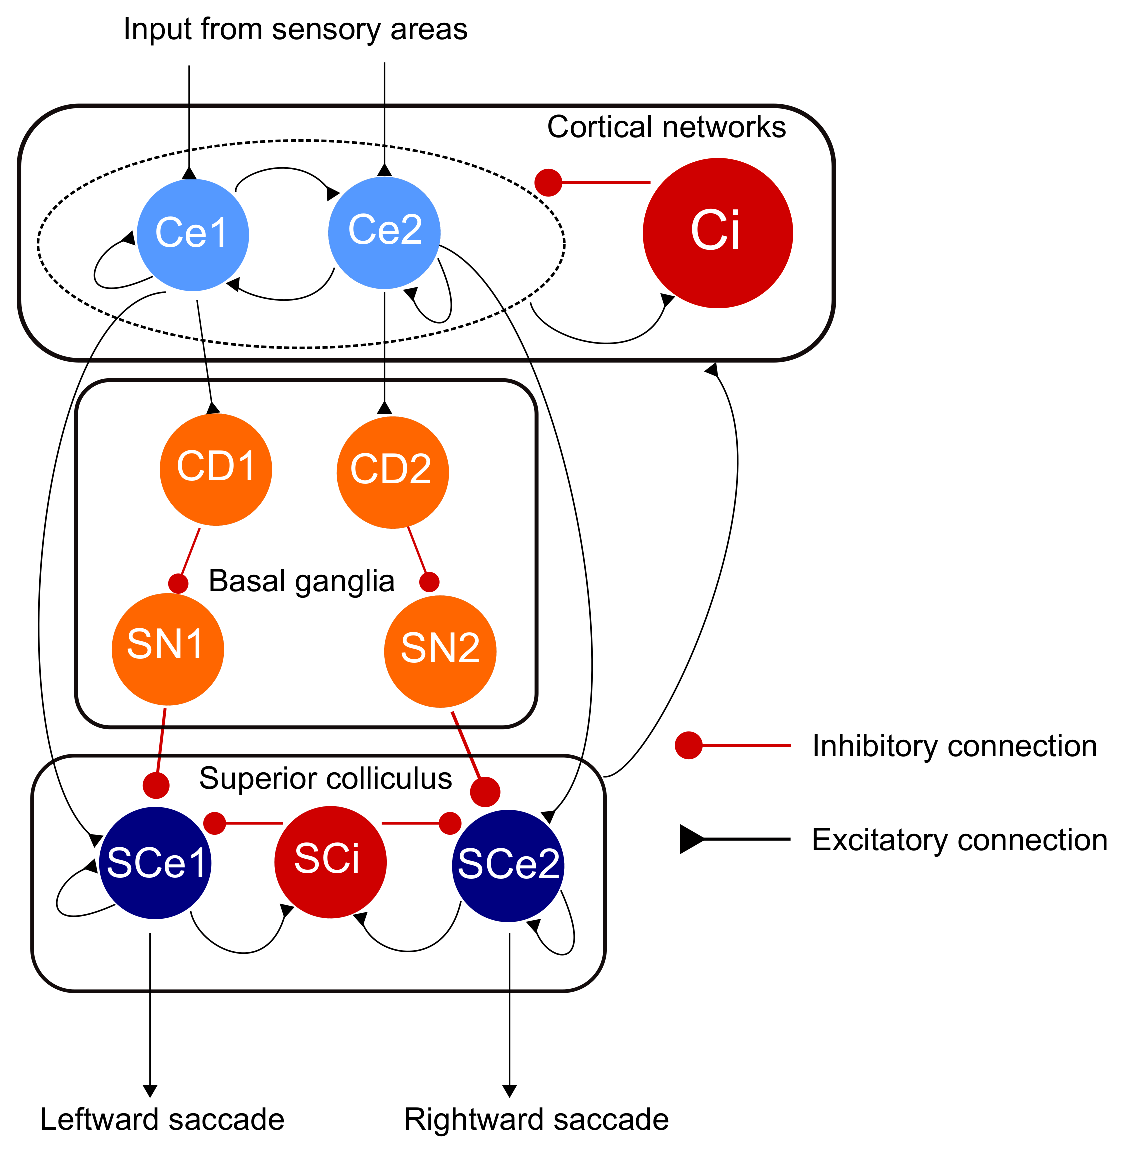
\includegraphics[width=0.8\linewidth]{Fig/Chapter1/Lo-Wang2006.eps}
	\caption{{\bf Model architecture of~\cite{lo2006cortico}.}  Neural pools in variation of blue represent excitatory pools and in variation of red it represents inhibitory populations. Neural pools in the cortical area receive a sensory input and compete through lateral inhibition due to interneurons. They project to caudate nucleus (CD) in the basal ganglia and superior colliculus (SC). The saccade and termination of the decision-making is performed by the superior colliculus that project back to cortical networks.   
	}
	\label{fig:rt-perf}
\end{figure}












%% une aprtie sur le DDM en neuroscience pure


%%% préciser que pas d'accord avec ce qu'il se dt dans la littérature sur l'équivalence DDM RNN % dans la conclusio nde la sous section peut être

%% préciser que un des problèmes de Wang c'est le fit, mais que maintenant on peut

%% Wang 2008 pour la partie sur l'attracteur


\section{What are the effects ... ?} %titre





%% conclusion de l'intro ?
%% RTs distribution modèles à atrtacteurs ?
%%

\end{comment}